\documentclass[10pt]{article}
\usepackage[margin=0.9in]{geometry}
\usepackage{amsmath,amssymb,mathtools}
\usepackage{graphicx}
\usepackage{hyperref}
\setlength{\parskip}{4pt}
\setlength{\parindent}{0pt}

\begin{document}
\begin{center}
{\Large FRC 100.005 — Thermodynamic Consistency of Resonant Collapse}\\
{\large October 2025}\\[4pt]
H. Servat
\\[4pt]
\small DOI: \href{https://doi.org/10.5281/zenodo.17438231}{10.5281/zenodo.17438231}
\end{center}

\section*{Abstract}
We show that a deterministic, resonance--based collapse mechanism (FRC 100.003) is consistent with the Second Law when measurements are modeled as open, dissipative processes. Local ordering (reduced uncertainty in the measured subsystem) is balanced by entropy export to the environment and the growth of system--environment correlations, so that total entropy increases. We give a minimal open--system model, derive qualitative accounting relations, and provide small, reproducible simulations that track $\Delta S_{\rm sys}$, $\Delta S_{\rm env}$, and mutual information $I(\mathrm{sys:env})$ during phase--locking to a pointer state.

\section*{1. Introduction}
Resonant phase--locking (FRC 100.003) treats measurement as an attractor selection. We address the thermodynamic requirement: does deterministic collapse violate the Second Law? Our answer is ``no'' in open systems: entropy exported to the environment and correlation growth ensure $\Delta S_{\rm total}\ge 0$.

\section*{2. Open--System Measurement}
Consider System + Apparatus + Environment with a pointer coupling. Define local entropies $S_{\rm sys}$, $S_{\rm app}$ and the environment contribution; include $I(\mathrm{sys:env})$ in accounting. Collapse reduces $S_{\rm sys}$ but increases $S_{\rm env}$ and $I(\mathrm{sys:env})$; in aggregate $\Delta S_{\rm total}\ge 0$.

\section*{3. Reciprocity Lens (optional)}
With $C=\exp[-S/k_*]$, local ordering corresponds to a coherence ascent $\Delta S\approx -k_*\Delta\ln C$. In open settings, reciprocity holds with exported entropy; see FRC 566.001.

\section*{4. Simulations (toy, reproducible)}
We simulate a two--level system with a pointer--like channel and an environment bath (effective dephasing). We track $S_{\rm sys}$, a proxy $S_{\rm env}$, and $I(\mathrm{sys:env})$ over time. Figures are generated by \verb|code/100.005/open_system_toy.py|.

\begin{center}
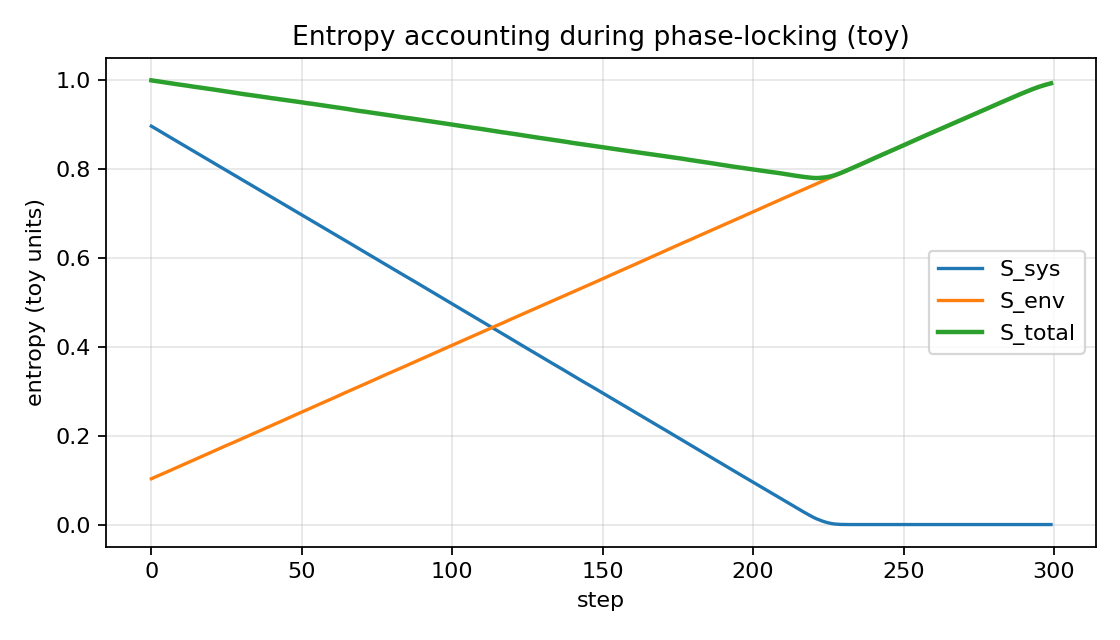
\includegraphics[width=0.75\linewidth]{entropy_accounting.png}\\
\emph{Figure 1.} Entropy accounting during phase--locking: local $S_{\rm sys}$ decreases while $S_{\rm env}$ increases; $\Delta S_{\rm total}\ge 0$.
\end{center}

\section*{5. Predictions}
\textbf{P--T1:} Mesoscopic readouts show small, reproducible dissipation bursts concurrent with locking.\newline
\textbf{P--T2:} Pre--collapse coherence ascent correlates with exported entropy rate in weak--measurement sequences.

\section*{6. Limits and Falsifiability}
Discuss closed--system limits, small drift regimes, and no--signaling. The program is falsifiable via P--T1 and P--T2.

\section*{Reproducibility}
Run \verb|python code/100.005/open_system_toy.py|; figures are written to \verb|artifacts/100.005/| with fixed seeds.

\section*{References}
\small
\begin{itemize}
  \item FRC~100.003 — Resonant Collapse (concept). DOI: \href{https://doi.org/10.5281/zenodo.15079820}{10.5281/zenodo.15079820}.
  \item FRC~566.001 — Reciprocity and UCC. DOI: \href{https://doi.org/10.5281/zenodo.17437759}{10.5281/zenodo.17437759}.
  \item FRC~100.003.566 — UCC \& Dissipation (Note). DOI: \href{https://doi.org/10.5281/zenodo.17437878}{10.5281/zenodo.17437878}.
\end{itemize}

\end{document}

